\documentclass[]{book}
\usepackage{lmodern}
\usepackage{amssymb,amsmath}
\usepackage{ifxetex,ifluatex}
\usepackage{fixltx2e} % provides \textsubscript
\ifnum 0\ifxetex 1\fi\ifluatex 1\fi=0 % if pdftex
  \usepackage[T1]{fontenc}
  \usepackage[utf8]{inputenc}
\else % if luatex or xelatex
  \ifxetex
    \usepackage{mathspec}
  \else
    \usepackage{fontspec}
  \fi
  \defaultfontfeatures{Ligatures=TeX,Scale=MatchLowercase}
\fi
% use upquote if available, for straight quotes in verbatim environments
\IfFileExists{upquote.sty}{\usepackage{upquote}}{}
% use microtype if available
\IfFileExists{microtype.sty}{%
\usepackage{microtype}
\UseMicrotypeSet[protrusion]{basicmath} % disable protrusion for tt fonts
}{}
\usepackage[margin=1in]{geometry}
\usepackage{hyperref}
\hypersetup{unicode=true,
            pdftitle={Biostatistics},
            pdfauthor={David Coffey},
            pdfborder={0 0 0},
            breaklinks=true}
\urlstyle{same}  % don't use monospace font for urls
\usepackage{natbib}
\bibliographystyle{apalike}
\usepackage{color}
\usepackage{fancyvrb}
\newcommand{\VerbBar}{|}
\newcommand{\VERB}{\Verb[commandchars=\\\{\}]}
\DefineVerbatimEnvironment{Highlighting}{Verbatim}{commandchars=\\\{\}}
% Add ',fontsize=\small' for more characters per line
\usepackage{framed}
\definecolor{shadecolor}{RGB}{248,248,248}
\newenvironment{Shaded}{\begin{snugshade}}{\end{snugshade}}
\newcommand{\KeywordTok}[1]{\textcolor[rgb]{0.13,0.29,0.53}{\textbf{#1}}}
\newcommand{\DataTypeTok}[1]{\textcolor[rgb]{0.13,0.29,0.53}{#1}}
\newcommand{\DecValTok}[1]{\textcolor[rgb]{0.00,0.00,0.81}{#1}}
\newcommand{\BaseNTok}[1]{\textcolor[rgb]{0.00,0.00,0.81}{#1}}
\newcommand{\FloatTok}[1]{\textcolor[rgb]{0.00,0.00,0.81}{#1}}
\newcommand{\ConstantTok}[1]{\textcolor[rgb]{0.00,0.00,0.00}{#1}}
\newcommand{\CharTok}[1]{\textcolor[rgb]{0.31,0.60,0.02}{#1}}
\newcommand{\SpecialCharTok}[1]{\textcolor[rgb]{0.00,0.00,0.00}{#1}}
\newcommand{\StringTok}[1]{\textcolor[rgb]{0.31,0.60,0.02}{#1}}
\newcommand{\VerbatimStringTok}[1]{\textcolor[rgb]{0.31,0.60,0.02}{#1}}
\newcommand{\SpecialStringTok}[1]{\textcolor[rgb]{0.31,0.60,0.02}{#1}}
\newcommand{\ImportTok}[1]{#1}
\newcommand{\CommentTok}[1]{\textcolor[rgb]{0.56,0.35,0.01}{\textit{#1}}}
\newcommand{\DocumentationTok}[1]{\textcolor[rgb]{0.56,0.35,0.01}{\textbf{\textit{#1}}}}
\newcommand{\AnnotationTok}[1]{\textcolor[rgb]{0.56,0.35,0.01}{\textbf{\textit{#1}}}}
\newcommand{\CommentVarTok}[1]{\textcolor[rgb]{0.56,0.35,0.01}{\textbf{\textit{#1}}}}
\newcommand{\OtherTok}[1]{\textcolor[rgb]{0.56,0.35,0.01}{#1}}
\newcommand{\FunctionTok}[1]{\textcolor[rgb]{0.00,0.00,0.00}{#1}}
\newcommand{\VariableTok}[1]{\textcolor[rgb]{0.00,0.00,0.00}{#1}}
\newcommand{\ControlFlowTok}[1]{\textcolor[rgb]{0.13,0.29,0.53}{\textbf{#1}}}
\newcommand{\OperatorTok}[1]{\textcolor[rgb]{0.81,0.36,0.00}{\textbf{#1}}}
\newcommand{\BuiltInTok}[1]{#1}
\newcommand{\ExtensionTok}[1]{#1}
\newcommand{\PreprocessorTok}[1]{\textcolor[rgb]{0.56,0.35,0.01}{\textit{#1}}}
\newcommand{\AttributeTok}[1]{\textcolor[rgb]{0.77,0.63,0.00}{#1}}
\newcommand{\RegionMarkerTok}[1]{#1}
\newcommand{\InformationTok}[1]{\textcolor[rgb]{0.56,0.35,0.01}{\textbf{\textit{#1}}}}
\newcommand{\WarningTok}[1]{\textcolor[rgb]{0.56,0.35,0.01}{\textbf{\textit{#1}}}}
\newcommand{\AlertTok}[1]{\textcolor[rgb]{0.94,0.16,0.16}{#1}}
\newcommand{\ErrorTok}[1]{\textcolor[rgb]{0.64,0.00,0.00}{\textbf{#1}}}
\newcommand{\NormalTok}[1]{#1}
\usepackage{longtable,booktabs}
\usepackage{graphicx,grffile}
\makeatletter
\def\maxwidth{\ifdim\Gin@nat@width>\linewidth\linewidth\else\Gin@nat@width\fi}
\def\maxheight{\ifdim\Gin@nat@height>\textheight\textheight\else\Gin@nat@height\fi}
\makeatother
% Scale images if necessary, so that they will not overflow the page
% margins by default, and it is still possible to overwrite the defaults
% using explicit options in \includegraphics[width, height, ...]{}
\setkeys{Gin}{width=\maxwidth,height=\maxheight,keepaspectratio}
\IfFileExists{parskip.sty}{%
\usepackage{parskip}
}{% else
\setlength{\parindent}{0pt}
\setlength{\parskip}{6pt plus 2pt minus 1pt}
}
\setlength{\emergencystretch}{3em}  % prevent overfull lines
\providecommand{\tightlist}{%
  \setlength{\itemsep}{0pt}\setlength{\parskip}{0pt}}
\setcounter{secnumdepth}{5}
% Redefines (sub)paragraphs to behave more like sections
\ifx\paragraph\undefined\else
\let\oldparagraph\paragraph
\renewcommand{\paragraph}[1]{\oldparagraph{#1}\mbox{}}
\fi
\ifx\subparagraph\undefined\else
\let\oldsubparagraph\subparagraph
\renewcommand{\subparagraph}[1]{\oldsubparagraph{#1}\mbox{}}
\fi

%%% Use protect on footnotes to avoid problems with footnotes in titles
\let\rmarkdownfootnote\footnote%
\def\footnote{\protect\rmarkdownfootnote}

%%% Change title format to be more compact
\usepackage{titling}

% Create subtitle command for use in maketitle
\newcommand{\subtitle}[1]{
  \posttitle{
    \begin{center}\large#1\end{center}
    }
}

\setlength{\droptitle}{-2em}

  \title{Biostatistics}
    \pretitle{\vspace{\droptitle}\centering\huge}
  \posttitle{\par}
    \author{David Coffey}
    \preauthor{\centering\large\emph}
  \postauthor{\par}
      \predate{\centering\large\emph}
  \postdate{\par}
    \date{2018-07-27}

\usepackage{booktabs}
\usepackage{amsthm}
\makeatletter
\def\thm@space@setup{%
  \thm@preskip=8pt plus 2pt minus 4pt
  \thm@postskip=\thm@preskip
}
\makeatother
\usepackage{booktabs}
\usepackage{longtable}
\usepackage{array}
\usepackage{multirow}
\usepackage[table]{xcolor}
\usepackage{wrapfig}
\usepackage{float}
\usepackage{colortbl}
\usepackage{pdflscape}
\usepackage{tabu}
\usepackage{threeparttable}
\usepackage{threeparttablex}
\usepackage[normalem]{ulem}
\usepackage{makecell}

\usepackage{amsthm}
\newtheorem{theorem}{Theorem}[chapter]
\newtheorem{lemma}{Lemma}[chapter]
\theoremstyle{definition}
\newtheorem{definition}{Definition}[chapter]
\newtheorem{corollary}{Corollary}[chapter]
\newtheorem{proposition}{Proposition}[chapter]
\theoremstyle{definition}
\newtheorem{example}{Example}[chapter]
\theoremstyle{definition}
\newtheorem{exercise}{Exercise}[chapter]
\theoremstyle{remark}
\newtheorem*{remark}{Remark}
\newtheorem*{solution}{Solution}
\begin{document}
\maketitle

{
\setcounter{tocdepth}{1}
\tableofcontents
}
\chapter{General overview}\label{general-overview}

\section{Introduction}\label{introduction}

This books provides a consise overview of biostatistics and its
applications using the R programming language. The textbook
\emph{Fundamentals of Biostatitics} \citep{Rosner2016} was used
extensivity in the preparation of this book.

\section{Example dataset}\label{example-dataset}

Examples of R functions are performed on a dataset of patients with
newly diagnosed multiple myeloma. This dataset contains a variety of
categorical and continuous variables. A description of the variables are
shown below.

\begin{tabular}{l|l}
\hline
Column & Description\\
\hline
ID & Patient identifier\\
\hline
Sex & Patient sex\\
\hline
Race & Patient race\\
\hline
Age & Patient age in years at the time of diagnosis\\
\hline
Stage & Disease stage according to the international staging system\\
\hline
SurvivalMonths & Duration in months between diagnosis and the last date of contact\\
\hline
Status & Survival status of the patient\\
\hline
DiagnosisYear & Year of diagnosis\\
\hline
Treatment & Initial treatment\\
\hline
TreatmentDurationMonths & Duration of the initial treatment in months\\
\hline
BonyLesions & Number of bony lesions on initial imaging study (MRI or X-ray)\\
\hline
PlasmaCells & Percentage of plasma cells on initial bone marrow biopsy\\
\hline
1q+ & FISH result on initial bone marrow biopsy\\
\hline
del13q & FISH result on initial bone marrow biopsy\\
\hline
del17p & FISH result on initial bone marrow biopsy\\
\hline
del1p & FISH result on initial bone marrow biopsy\\
\hline
t(11;14) & FISH result on initial bone marrow biopsy\\
\hline
t(14;16) & FISH result on initial bone marrow biopsy\\
\hline
t(4:14) & FISH result on initial bone marrow biopsy\\
\hline
t(6;14) & FISH result on initial bone marrow biopsy\\
\hline
Albumin & Albumin  at the time of diagnosis\\
\hline
B2M & Beta-2 microglobulin at the time of diagnosis\\
\hline
Calcium & Calcium at the time of diagnosis\\
\hline
Creatinine & Creatinine at the time of diagnosis\\
\hline
LightChainRatio & Involved/uninvolved serum free light chain ratio at the time of diagnosis\\
\hline
Hematocrit & Hematocrit at the time of diagnosis\\
\hline
LDH & Lactate dehydrogenase at the time of diagnosis\\
\hline
MProtein & Monoclonal protein at the time of diagnosis\\
\hline
\end{tabular}

\chapter{Descriptive statistics}\label{descriptive-statistics}

\section{Measures of location}\label{measures-of-location}

\subsection{Arithmetic mean}\label{arithmetic-mean}

The arithmetic mean (\(\bar{x}\)) is a measure of central location. It
is calculated from the sum of all the observations (\({n}\)) divided by
the number of observations:

\[\bar{x}=\frac{\sum_{i=1}^nx_{i}}{n}\]

The notation \(\sum_{i=1}^nx_{i}\) means the sum of all \({x}_i\)
observations \(({x}_1+{x}_2+{x}_n)\). One limitation to the arithmetic
mean is that it is overly sensitive to extreme values.

\begin{Shaded}
\begin{Highlighting}[]
\CommentTok{# Import dataset}
\KeywordTok{load}\NormalTok{(}\StringTok{"docs/Example-data.Rda"}\NormalTok{)}

\CommentTok{# Calcuate arithmetic mean}
\KeywordTok{mean}\NormalTok{(data}\OperatorTok{$}\NormalTok{Age)}
\end{Highlighting}
\end{Shaded}

\begin{verbatim}
[1] 59.5
\end{verbatim}

\subsection{Median}\label{median}

If all observations are ordered from smallest to largest, the median is
the middle number. More precisely, if \({n}\) is odd, \(\frac{n+1}{2}\),
or if \({n}\) is even, the average of \(\frac{n}{2}\) and
\(\frac{n}{2}+1\). The rationale for using to the median is to ensure an
equal number of observations on both sides of the sample median. The
main weakness of the sample median is that it is less sensitive to the
actual numeric values of the data points. If the sample distribution is
symmetric, the arithmetic mean is approximately the same as the median.
For positively skewed distributions, the arithmetic mean tends to be
larger than the median; for negatively skewed distributions, the
arithmetic means tends to be smaller than the median.

\begin{Shaded}
\begin{Highlighting}[]
\CommentTok{# Calcuate arithmetic mean}
\KeywordTok{median}\NormalTok{(data}\OperatorTok{$}\NormalTok{Age)}
\end{Highlighting}
\end{Shaded}

\begin{verbatim}
[1] 62.5
\end{verbatim}

\subsection{Mode}\label{mode}

The mode is the most frequently occurring value among all of the
observations in a sample. Some distributions have more than one mode. A
distribution with one mode is called unimodal; two modes, bimodal; three
modes, trimodal.

\begin{Shaded}
\begin{Highlighting}[]
\CommentTok{# Calcuate mode}
\KeywordTok{library}\NormalTok{(DescTools)}
\KeywordTok{Mode}\NormalTok{(data}\OperatorTok{$}\NormalTok{Age)}
\end{Highlighting}
\end{Shaded}

\begin{verbatim}
[1] 64
\end{verbatim}

\subsection{Geometric mean}\label{geometric-mean}

The geometric mean (\(\bar{logx}\)) is the central number in a geometric
progression such as exponential growth. The geometric mean is defined as
the \({n}\)th root of the product of \({n}\) numbers:

\[\bar{logx}=\frac{\sum_{i=1}^nlogx_{i}}{n}\] Any base can be used to
compute the logarithms for the geometric mean. It is usually preferable
to work in the original scale by taking the antilogarithm of
\(\bar{logx}\) to form the geometric mean.

\begin{Shaded}
\begin{Highlighting}[]
\CommentTok{# Calcuate geometric arithmetic mean}
\KeywordTok{library}\NormalTok{(DescTools)}
\KeywordTok{Gmean}\NormalTok{(data}\OperatorTok{$}\NormalTok{Age)}
\end{Highlighting}
\end{Shaded}

\begin{verbatim}
[1] 58.61499
\end{verbatim}

\section{Measures of spread}\label{measures-of-spread}

\subsection{Range}\label{range}

The range is the difference between the smallest and largest
observations in a sample. Range is very sensitive to extreme
observations and depends on the sample size since the large the \({n}\),
the largest the range tends to be.

\begin{Shaded}
\begin{Highlighting}[]
\CommentTok{# Calcuate range}
\KeywordTok{range}\NormalTok{(data}\OperatorTok{$}\NormalTok{Age)}
\end{Highlighting}
\end{Shaded}

\begin{verbatim}
[1] 33 76
\end{verbatim}

\subsection{Percentile}\label{percentile}

Percentile is the value below which a given percentage of observations
in a group of observations fall. The median is the 50th percentile and
is a special case of a quantile. Compared to range, percentiles are less
sensitive to outliers. The \({p}\)th percentile is defined by the
\({(k+1)}\)th largest sample observation if \({np/100}\) is not an
integer where \({k}\) is the largest integer less than \({np/100}\). If
\({np/100}\) is an integer, then the \({p}\)th percentile is the average
of the \({(np/100)}\)th and the \({(np/100+1)}\)th largest observations.

\begin{Shaded}
\begin{Highlighting}[]
\CommentTok{# Calcuate the 5th and 95th percentiles}
\KeywordTok{quantile}\NormalTok{(data}\OperatorTok{$}\NormalTok{Age, }\DataTypeTok{probs =} \KeywordTok{c}\NormalTok{(}\FloatTok{0.05}\NormalTok{, }\FloatTok{0.95}\NormalTok{), }\DataTypeTok{type =} \DecValTok{2}\NormalTok{)}
\end{Highlighting}
\end{Shaded}

\begin{verbatim}
  5%  95% 
38.5 74.0 
\end{verbatim}

\subsection{Variance}\label{variance}

Variance (\({s^2}\)) is the average of the squared differences from the
mean. The reason for squaring the differences is because the sum of the
differences are always equal to zero.
\[{s^2=\frac{\sum_{i=1}^n(x_i-\bar{x})^2}{n-1}}\]

\begin{Shaded}
\begin{Highlighting}[]
\CommentTok{# Calcuate variance}
\KeywordTok{var}\NormalTok{(data}\OperatorTok{$}\NormalTok{Age)}
\end{Highlighting}
\end{Shaded}

\begin{verbatim}
[1] 95.31579
\end{verbatim}

\subsection{Standard deviation}\label{standard-deviation}

Standard deviation (\({s}\)) is the square root of the sample variance.
The advantage of using the standard deviation over the variance is that
both the mean and standard deviation are in the same units whereas the
variance and mean are not.
\[{s=\sqrt\frac{\sum_{i=1}^n(x_i-\bar{x})^2}{n-1}}\]

\begin{Shaded}
\begin{Highlighting}[]
\CommentTok{# Calcuate standard deviation}
\KeywordTok{sd}\NormalTok{(data}\OperatorTok{$}\NormalTok{Age)}
\end{Highlighting}
\end{Shaded}

\begin{verbatim}
[1] 9.762981
\end{verbatim}

\subsection{Standard error of the
mean}\label{standard-error-of-the-mean}

The standard error (\({se}\)) of the mean is how far the sample mean
deviates from the population mean. It is equal to the variance obtained
from a set of sample means from repeated samples of size \({n}\) from a
population with underlying variance \({s}\). The standard error of the
mean is estimated by \(\frac{s}{\sqrt{n}}\). The larger the sample size,
the more precise the sample mean will estimate the population mean.

\begin{Shaded}
\begin{Highlighting}[]
\CommentTok{# Calcuate standard error}
\KeywordTok{library}\NormalTok{(DescTools)}
\KeywordTok{MeanSE}\NormalTok{(data}\OperatorTok{$}\NormalTok{Age)}
\end{Highlighting}
\end{Shaded}

\begin{verbatim}
[1] 2.183069
\end{verbatim}

\subsection{Coefficient of varaince}\label{coefficient-of-varaince}

The coefficient of variation (\({CV}\)) is a measure of relative
variability and remains the same regardless of the observations units.
\({CV}\) is defined by \({100\% \times s/\bar{x}}\). Coefficient of
variation is most useful in comparing the variability of several
different samples, each with different arithmetic means.

\begin{Shaded}
\begin{Highlighting}[]
\CommentTok{# Calcuate coefficient of variance}
\KeywordTok{library}\NormalTok{(DescTools)}
\KeywordTok{CoefVar}\NormalTok{(data}\OperatorTok{$}\NormalTok{Age)}
\end{Highlighting}
\end{Shaded}

\begin{verbatim}
[1] 0.1640837
\end{verbatim}

\section{Visualizing descriptive
statistics}\label{visualizing-descriptive-statistics}

\subsection{Single variable}\label{single-variable}

\subsubsection{Stem and leaf plot}\label{stem-and-leaf-plot}

\begin{Shaded}
\begin{Highlighting}[]
\CommentTok{# Create a stem and leaf plot}
\KeywordTok{stem}\NormalTok{(data}\OperatorTok{$}\NormalTok{Age)}
\end{Highlighting}
\end{Shaded}

\begin{verbatim}

  The decimal point is 1 digit(s) to the right of the |

  3 | 3
  4 | 4
  5 | 123578
  6 | 0234444459
  7 | 26
\end{verbatim}

\subsubsection{Frequency distribution
table}\label{frequency-distribution-table}

\begin{Shaded}
\begin{Highlighting}[]
\CommentTok{# Create a frequency distribution table}
\KeywordTok{table}\NormalTok{(data}\OperatorTok{$}\NormalTok{Age)}
\end{Highlighting}
\end{Shaded}

\begin{verbatim}

33 44 51 52 53 55 57 58 60 62 63 64 65 69 72 76 
 1  1  1  1  1  1  1  1  1  1  1  5  1  1  1  1 
\end{verbatim}

\subsubsection{Dot plot}\label{dot-plot}

\begin{Shaded}
\begin{Highlighting}[]
\CommentTok{# Create a dot plot}
\KeywordTok{library}\NormalTok{(ggplot2)}
\KeywordTok{ggplot}\NormalTok{(}\DataTypeTok{data =}\NormalTok{ data, }\KeywordTok{aes}\NormalTok{(}\DataTypeTok{x =}\NormalTok{ Age)) }\OperatorTok{+}
\StringTok{  }\KeywordTok{geom_dotplot}\NormalTok{()}
\end{Highlighting}
\end{Shaded}

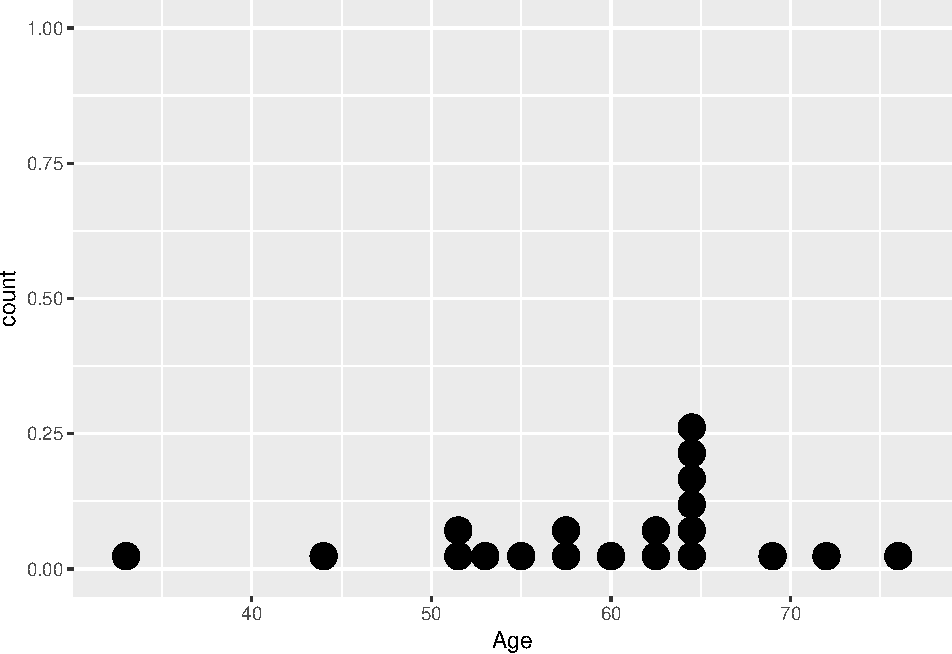
\includegraphics{Biostatistics_files/figure-latex/unnamed-chunk-14-1.pdf}

\subsubsection{Histogram}\label{histogram}

\begin{Shaded}
\begin{Highlighting}[]
\CommentTok{# Create a histogram}
\KeywordTok{library}\NormalTok{(ggplot2)}
\KeywordTok{ggplot}\NormalTok{(}\DataTypeTok{data =}\NormalTok{ data, }\KeywordTok{aes}\NormalTok{(}\DataTypeTok{x =}\NormalTok{ Age)) }\OperatorTok{+}
\StringTok{  }\KeywordTok{geom_histogram}\NormalTok{()}
\end{Highlighting}
\end{Shaded}

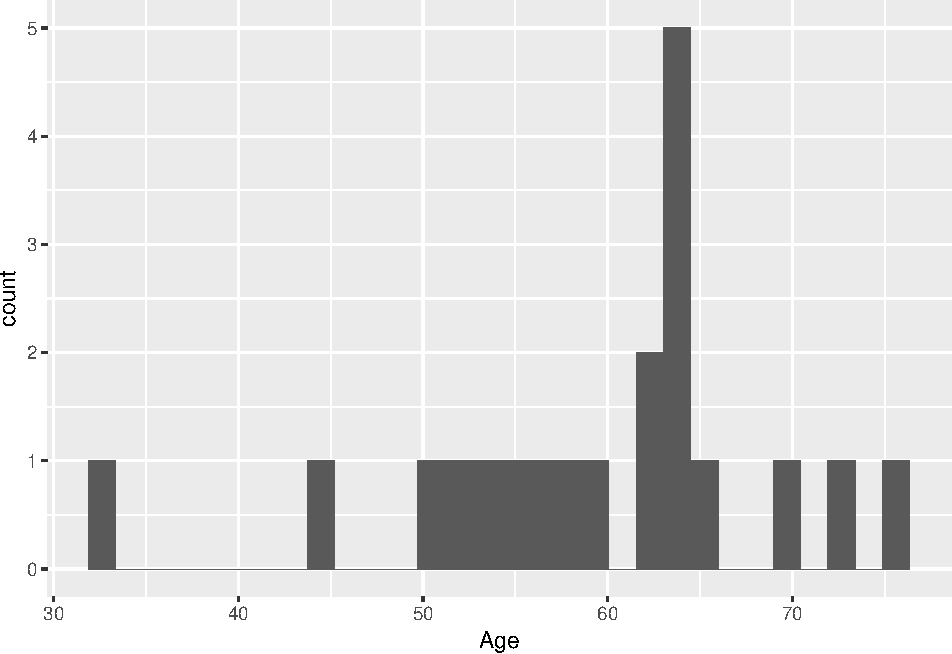
\includegraphics{Biostatistics_files/figure-latex/unnamed-chunk-15-1.pdf}

\subsubsection{Density plot}\label{density-plot}

\begin{Shaded}
\begin{Highlighting}[]
\CommentTok{# Create a density plot}
\KeywordTok{library}\NormalTok{(ggplot2)}
\KeywordTok{ggplot}\NormalTok{(}\DataTypeTok{data =}\NormalTok{ data, }\KeywordTok{aes}\NormalTok{(}\DataTypeTok{x =}\NormalTok{ Age)) }\OperatorTok{+}
\StringTok{  }\KeywordTok{geom_density}\NormalTok{()}
\end{Highlighting}
\end{Shaded}

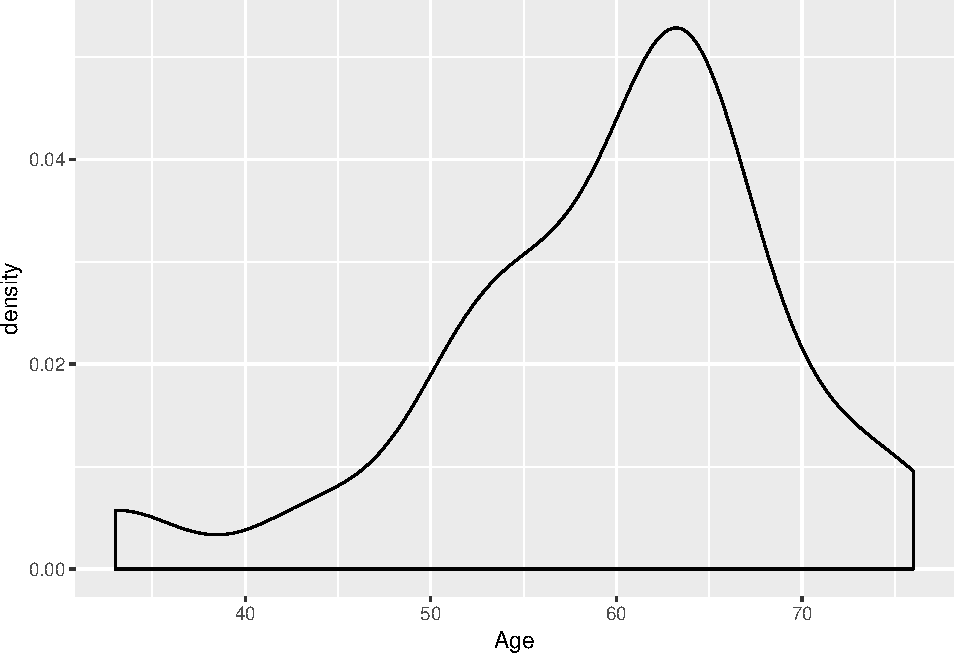
\includegraphics{Biostatistics_files/figure-latex/unnamed-chunk-16-1.pdf}

\subsection{Muliple variables}\label{muliple-variables}

\subsubsection{Summary table}\label{summary-table}

\begin{Shaded}
\begin{Highlighting}[]
\CommentTok{# Create a summary statistics table}
\KeywordTok{library}\NormalTok{(dplyr)}
\NormalTok{stats <-}\StringTok{ }\KeywordTok{group_by}\NormalTok{(data, Sex) }\OperatorTok
\KeywordTok{summarise}\NormalTok{(}\DataTypeTok{Mean =} \KeywordTok{mean}\NormalTok{(Age), }\DataTypeTok{Median =} \KeywordTok{median}\NormalTok{(Age), }\DataTypeTok{SD =} \KeywordTok{sd}\NormalTok{(Age), }\DataTypeTok{SE =} \KeywordTok{MeanSE}\NormalTok{(Age), }\DataTypeTok{N =} \KeywordTok{n}\NormalTok{())}
\NormalTok{stats}
\end{Highlighting}
\end{Shaded}

\begin{verbatim}
# A tibble: 2 x 6
  Sex     Mean Median    SD    SE     N
  <fct>  <dbl>  <dbl> <dbl> <dbl> <int>
1 Female  57.9   63   12.8   4.52     8
2 Male    60.6   60.5  7.57  2.19    12
\end{verbatim}

\subsubsection{Bar graph}\label{bar-graph}

\begin{Shaded}
\begin{Highlighting}[]
\CommentTok{# Create a bar graph with standard error bars}
\KeywordTok{library}\NormalTok{(ggplot2)}
\KeywordTok{ggplot}\NormalTok{(}\DataTypeTok{data =}\NormalTok{ stats, }\KeywordTok{aes}\NormalTok{(}\DataTypeTok{x =}\NormalTok{ Sex, }\DataTypeTok{y =}\NormalTok{ Mean)) }\OperatorTok{+}
\StringTok{  }\KeywordTok{geom_bar}\NormalTok{(}\DataTypeTok{stat =} \StringTok{"identity"}\NormalTok{) }\OperatorTok{+}
\StringTok{  }\KeywordTok{geom_errorbar}\NormalTok{(}\KeywordTok{aes}\NormalTok{(}\DataTypeTok{ymin =}\NormalTok{ Mean}\OperatorTok{-}\NormalTok{SE, }\DataTypeTok{ymax =}\NormalTok{ Mean}\OperatorTok{+}\NormalTok{SE, }\DataTypeTok{width =} \FloatTok{0.2}\NormalTok{)) }\OperatorTok{+}
\StringTok{  }\KeywordTok{labs}\NormalTok{(}\DataTypeTok{y =} \StringTok{"Mean age"}\NormalTok{)}
\end{Highlighting}
\end{Shaded}

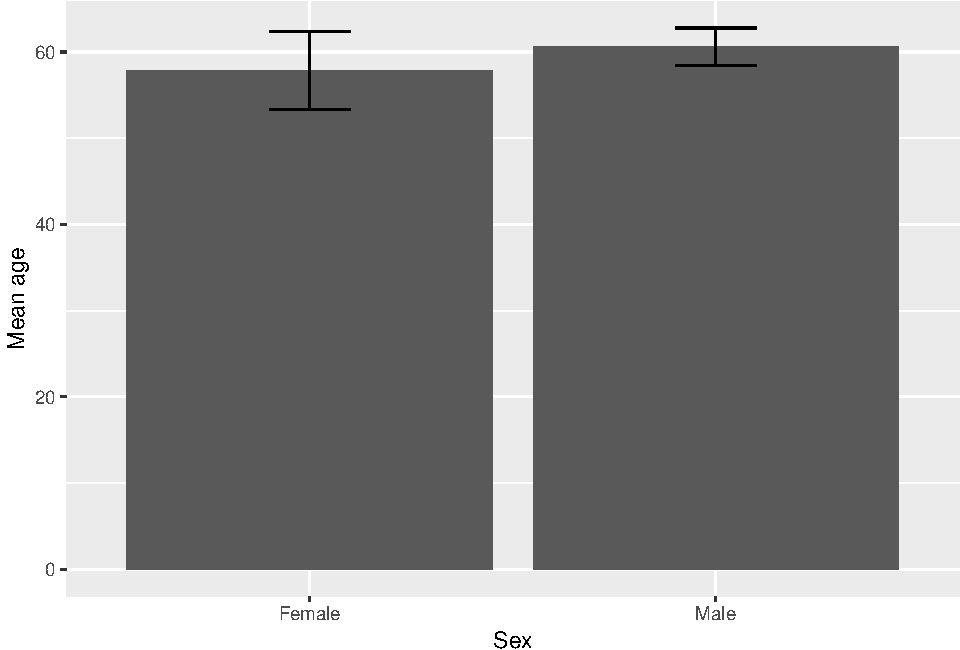
\includegraphics{Biostatistics_files/figure-latex/unnamed-chunk-19-1.pdf}

\subsubsection{Box plot}\label{box-plot}

\begin{Shaded}
\begin{Highlighting}[]
\CommentTok{# Create a boxplot}
\KeywordTok{library}\NormalTok{(ggplot2)}
\KeywordTok{ggplot}\NormalTok{(}\DataTypeTok{data =}\NormalTok{ data, }\KeywordTok{aes}\NormalTok{(}\DataTypeTok{x =}\NormalTok{ Sex, }\DataTypeTok{y =}\NormalTok{ Age)) }\OperatorTok{+}
\StringTok{  }\KeywordTok{geom_boxplot}\NormalTok{()}
\end{Highlighting}
\end{Shaded}

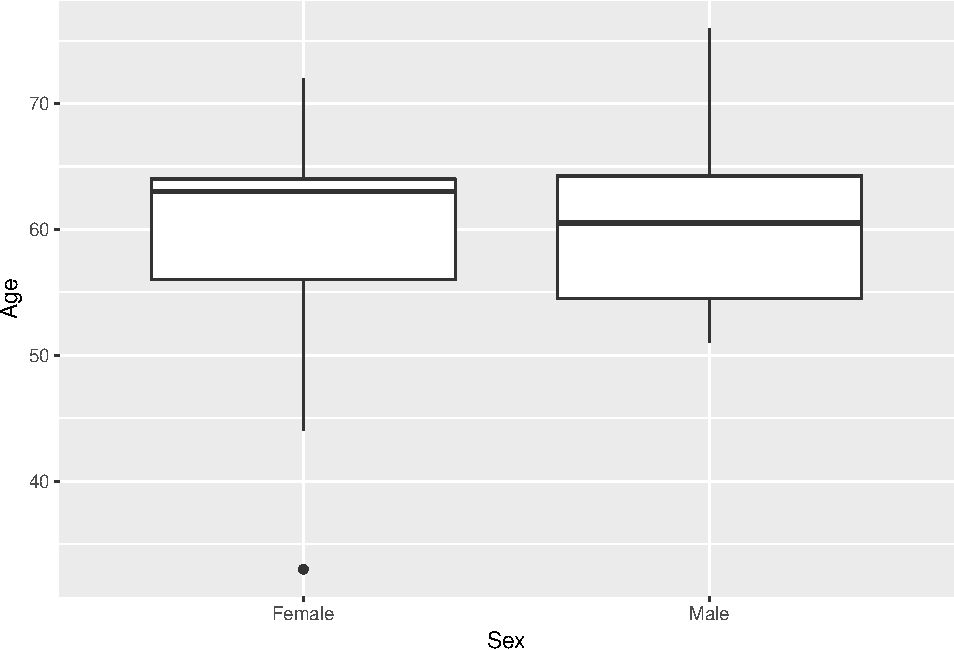
\includegraphics{Biostatistics_files/figure-latex/unnamed-chunk-20-1.pdf}

\subsubsection{Violin plot}\label{violin-plot}

\begin{Shaded}
\begin{Highlighting}[]
\CommentTok{# Create a violin plot}
\KeywordTok{library}\NormalTok{(ggplot2)}
\KeywordTok{ggplot}\NormalTok{(}\DataTypeTok{data =}\NormalTok{ data, }\KeywordTok{aes}\NormalTok{(}\DataTypeTok{x =}\NormalTok{ Sex, }\DataTypeTok{y =}\NormalTok{ Age)) }\OperatorTok{+}
\StringTok{  }\KeywordTok{geom_violin}\NormalTok{()}
\end{Highlighting}
\end{Shaded}

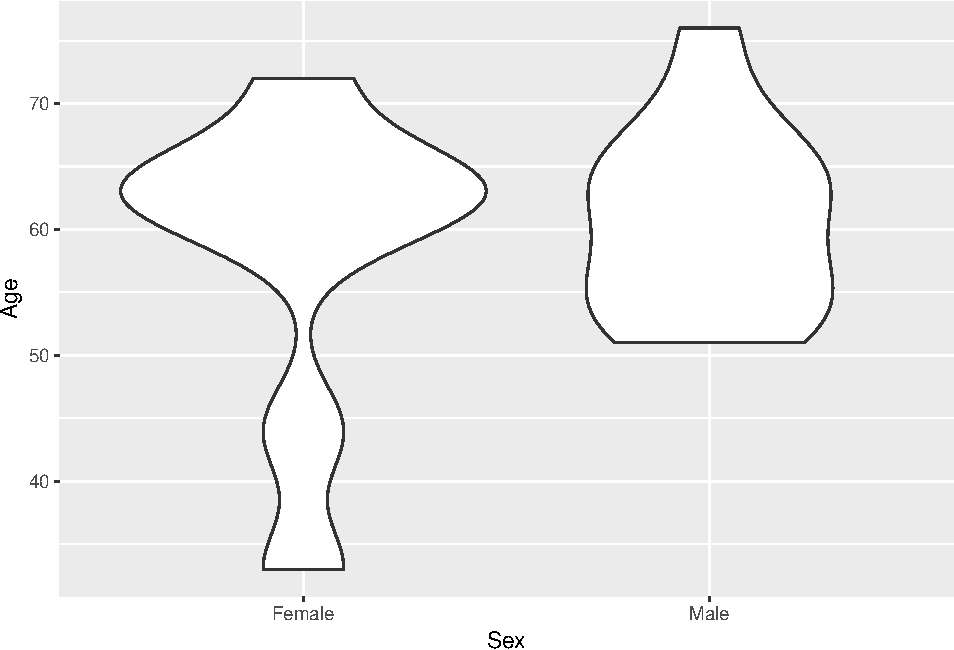
\includegraphics{Biostatistics_files/figure-latex/unnamed-chunk-21-1.pdf}

\subsubsection{Jitter plot}\label{jitter-plot}

\begin{Shaded}
\begin{Highlighting}[]
\CommentTok{# Create a jitter plot}
\KeywordTok{library}\NormalTok{(ggplot2)}
\KeywordTok{ggplot}\NormalTok{(}\DataTypeTok{data =}\NormalTok{ data, }\KeywordTok{aes}\NormalTok{(}\DataTypeTok{x =}\NormalTok{ Sex, }\DataTypeTok{y =}\NormalTok{ Age)) }\OperatorTok{+}
\StringTok{  }\KeywordTok{geom_jitter}\NormalTok{(}\DataTypeTok{width =} \FloatTok{0.2}\NormalTok{)}
\end{Highlighting}
\end{Shaded}

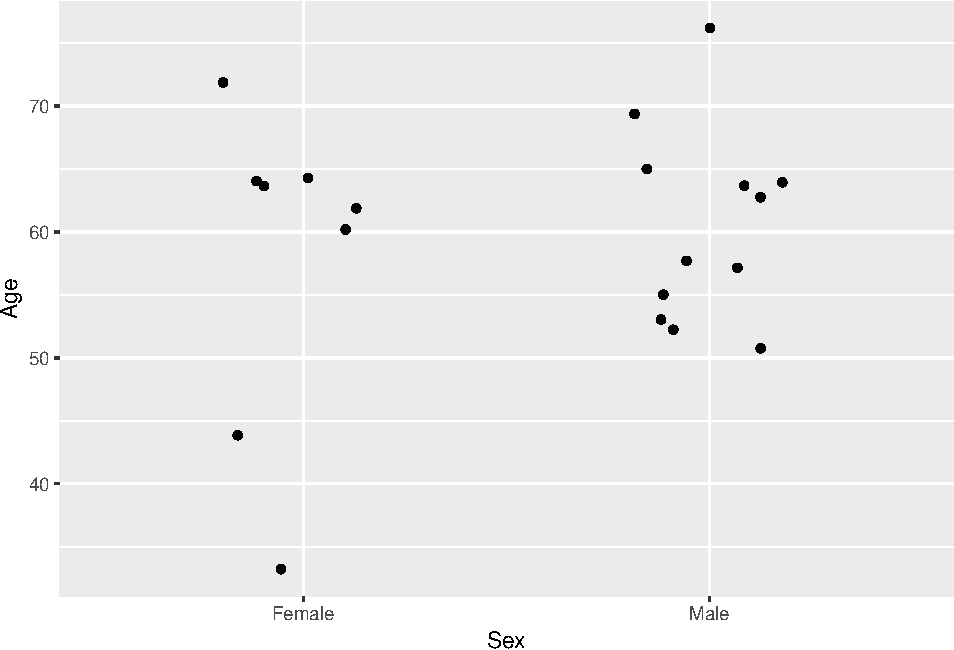
\includegraphics{Biostatistics_files/figure-latex/unnamed-chunk-22-1.pdf}

\chapter{Probability}\label{probability}

\section{Table of confusion}\label{table-of-confusion}

A table of confusion is a table with 2 rows and 2 columns that reports
the number of false positives, false negatives, true positives, and true
negatives. Rows represent a prediction outcomes such as a test result
and columns represent outcomes of the condition being predicted such as
a disease state.

\begin{Shaded}
\begin{Highlighting}[]
\CommentTok{# Import dataset}
\KeywordTok{load}\NormalTok{(}\StringTok{"docs/Example-data.Rda"}\NormalTok{)}

\CommentTok{# Create a table of confusion}
\NormalTok{BonyLesions <-}\StringTok{ }\KeywordTok{ifelse}\NormalTok{(data}\OperatorTok{$}\NormalTok{BonyLesions }\OperatorTok{!=}\StringTok{ "0"}\NormalTok{ , }\StringTok{"Abnormal"}\NormalTok{, }\StringTok{"Normal"}\NormalTok{)}
\NormalTok{MProtein <-}\StringTok{ }\KeywordTok{ifelse}\NormalTok{(data}\OperatorTok{$}\NormalTok{MProtein }\OperatorTok{>}\StringTok{ }\DecValTok{0}\NormalTok{ , }\StringTok{"Abnormal"}\NormalTok{, }\StringTok{"Normal"}\NormalTok{)}
\KeywordTok{table}\NormalTok{(MProtein, BonyLesions)}
\end{Highlighting}
\end{Shaded}

\begin{verbatim}
          BonyLesions
MProtein   Abnormal Normal
  Abnormal        9      6
  Normal          4      1
\end{verbatim}

Sensitivity and specificity to assess the quality of a test. Positive
and negative predictive values to interpret the results of the test.

\section{Sensitivity}\label{sensitivity}

Sensitivity is the ability of a test to correctly classify an individual
as having a disease. It is defined by the probability of having a
positive test when the disease is present:
\[{\frac{True\ positives}{True\ positives + False\ negatives}=\frac{True\ positives}{Number\ with\ condition}}\]

\begin{Shaded}
\begin{Highlighting}[]
\CommentTok{# Calculate sensitivity}
\KeywordTok{library}\NormalTok{(caret)}
\KeywordTok{sensitivity}\NormalTok{(}\KeywordTok{factor}\NormalTok{(MProtein), }\KeywordTok{factor}\NormalTok{(BonyLesions)) }\CommentTok{# sensitivity(prediction,truth)}
\end{Highlighting}
\end{Shaded}

\begin{verbatim}
[1] 0.6923077
\end{verbatim}

\section{Specificity}\label{specificity}

Specificity is the ability of a test to correctly classify an individual
disease free. It is defined by the probability of having a negative test
when the disease absent:
\[{\frac{True\ negatives}{True\ negatives + False\ positives}=\frac{True\ negatives}{Number\ without\ condition}}\]

\begin{Shaded}
\begin{Highlighting}[]
\CommentTok{# Calculate specificity}
\KeywordTok{library}\NormalTok{(caret)}
\KeywordTok{specificity}\NormalTok{(}\KeywordTok{factor}\NormalTok{(MProtein), }\KeywordTok{factor}\NormalTok{(BonyLesions)) }\CommentTok{# specificity(prediction,truth)}
\end{Highlighting}
\end{Shaded}

\begin{verbatim}
[1] 0.1428571
\end{verbatim}

\section{Postitive predictive value}\label{postitive-predictive-value}

Positive predictive value is the percentage of patients with a positive
test who actually have the disease. It is defined by the probability of
having the disease when the test is positive:
\[{\frac{True\ positives}{True\ positives + False\ positives}=\frac{True\ positives}{Postive\ predictions}}\]

\begin{Shaded}
\begin{Highlighting}[]
\CommentTok{# Calculate postitive predictive value}
\KeywordTok{library}\NormalTok{(caret)}
\KeywordTok{posPredValue}\NormalTok{(}\KeywordTok{factor}\NormalTok{(MProtein), }\KeywordTok{factor}\NormalTok{(BonyLesions)) }\CommentTok{# posPredValue(prediction,truth)}
\end{Highlighting}
\end{Shaded}

\begin{verbatim}
[1] 0.6
\end{verbatim}

\section{Negative predictive value}\label{negative-predictive-value}

Negative predictive value is the percentage of patients with a negative
test who do not have the disease. It is defined by the probability of
not having the disease when the test is negative:
\[{\frac{True\ negataives}{True\ negatives + False\ negatives}=\frac{True\ positives}{Negative\ predictions}}\]

\begin{Shaded}
\begin{Highlighting}[]
\CommentTok{# Calculate negative predictive value}
\KeywordTok{library}\NormalTok{(caret)}
\KeywordTok{negPredValue}\NormalTok{(}\KeywordTok{factor}\NormalTok{(MProtein), }\KeywordTok{factor}\NormalTok{(BonyLesions)) }\CommentTok{# negPredValue(prediction,truth)}
\end{Highlighting}
\end{Shaded}

\begin{verbatim}
[1] 0.2
\end{verbatim}

\section{ROC curve}\label{roc-curve}

The receiver operating characteristics (ROC) curve is a plot of the true
positive rate versus (sensitivity) versus the false positive rate
(specificity) of a screening test. Each point on the curve corresponds
to different cutoff points used to designate a positive test. The area
under the curve is an estimate of the accuracy of the test.

\begin{Shaded}
\begin{Highlighting}[]
\KeywordTok{library}\NormalTok{(plotROC)}
\KeywordTok{library}\NormalTok{(ggplot2)}

\KeywordTok{ggplot}\NormalTok{(}\KeywordTok{data.frame}\NormalTok{(BonyLesions, }\DataTypeTok{MProtein =}\NormalTok{ data}\OperatorTok{$}\NormalTok{MProtein), }\KeywordTok{aes}\NormalTok{(}\DataTypeTok{d =}\NormalTok{ BonyLesions, }\DataTypeTok{m =}\NormalTok{ MProtein)) }\OperatorTok{+}\StringTok{ }
\StringTok{  }\KeywordTok{geom_roc}\NormalTok{() }\OperatorTok{+}
\StringTok{  }\KeywordTok{style_roc}\NormalTok{()}
\end{Highlighting}
\end{Shaded}

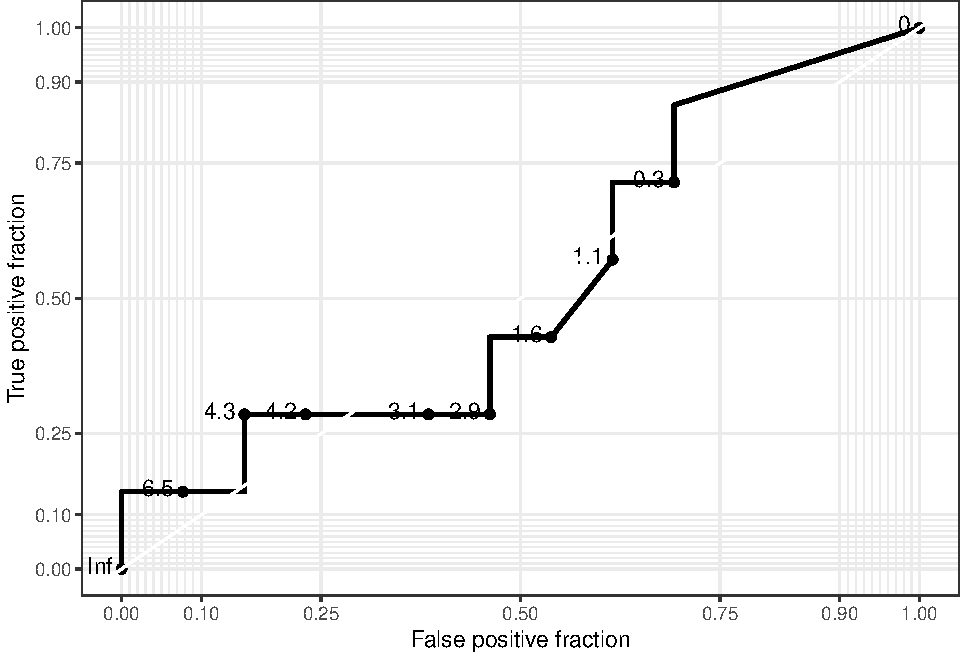
\includegraphics{Biostatistics_files/figure-latex/unnamed-chunk-28-1.pdf}

\begin{Shaded}
\begin{Highlighting}[]
\CommentTok{# Calculate area under the curve}
\KeywordTok{calc_auc}\NormalTok{(}
  \KeywordTok{ggplot}\NormalTok{(}\KeywordTok{data.frame}\NormalTok{(BonyLesions, }\DataTypeTok{MProtein =}\NormalTok{ data}\OperatorTok{$}\NormalTok{MProtein), }\KeywordTok{aes}\NormalTok{(}\DataTypeTok{d =}\NormalTok{ BonyLesions, }\DataTypeTok{m =}\NormalTok{ MProtein)) }\OperatorTok{+}\StringTok{ }
\StringTok{    }\KeywordTok{geom_roc}\NormalTok{()}
\NormalTok{  )}
\end{Highlighting}
\end{Shaded}

\begin{verbatim}
  PANEL group      AUC
1     1    -1 0.521978
\end{verbatim}

\section{Baysian inference}\label{baysian-inference}

Frequentist inference is a type of statistical inference that draws
conclusions from sample data by emphasizing the frequency or proportion
of the data. Bayesian inference is an alternative method of statistical
inference in which Bayes' theorem is used to update the probability for
a hypothesis as more evidence or information becomes available. It is
given by the following formula:
\[Baye's\ theorem = {Pr({A|B})=\frac{Pr(B|A)\times Pr(A)}{Pr(B)}}\]
where \({Pr({A|B})}\) the likelihood of event \({A}\) occurring given
that \({B}\) is true, \({Pr({B|A})}\) the likelihood of event \({B}\)
occurring given that \({A}\) is true, and \({Pr({A)}}\) and \({Pr(A)}\)
are the probabilities of observing A and B independently of each other.
Bayesians conceive of two types of probability, a \textbf{prior
probability} of an event which is the best guess by the observer in the
absence of data, and a \textbf{posterior probability} which is the
likelihood that an event will occur after collecting some empirical
data.

\chapter{Normal distribution}\label{normal-distribution}

\section{Probability distributions}\label{probability-distributions}

A probability distribution is a mathematical function that provides the
probabilities of occurrence of different possible outcomes. Probability
distributions are generally divided into two classes. A \textbf{discrete
probability distribution} applies to discrete random variables such as
the probability of being alive or dead as in the binomial distribution
or the probability of a given number of deaths occurring in a fixed time
interval as in the Poisson distribution. A \textbf{continuous
probability distribution} applies to continuous random variables such as
the measure of hematocrit on any given day. The most common continuous
probability distribution is the normal or Gaussian distribution and is
defined by the following probability-density function:
\[f(x)=\frac{1}{\sqrt{2\pi\sigma}}e^{-\frac{1}{2\sigma^{2}}(x-\mu)^{2}}\]
where \({x}\) is a continuous random variable, \({\sigma^{2}}\) is the
variance, and \({\mu}\) is the mean. Properties of the normal
distribution include:

\begin{itemize}
\tightlist
\item
  The curve is symmetric about \({\mu}\)
\item
  The entire shape of the normal distribution is determined by the two
  parameters \({\mu}\) and \({\sigma^{2}}\)
\item
  The area under the curve between any two points \({a}\) and \({b}\) is
  equal to the probability that the random variable \({x}\) falls
  between \({a}\) and \({b}\)
\item
  The area under the entire normal density function is always equal to 1
\item
  The probability that the random variable \({x}\) falls between ±1
  standard deviation is approximately 68\%, ±2 standard deviations is
  95\%, and ±2.5 standard deviations is 99\%.
\end{itemize}

\begin{Shaded}
\begin{Highlighting}[]
\CommentTok{# Calculate the probabilities of a normally distributed random variable}
\KeywordTok{library}\NormalTok{(ggplot2)}
\NormalTok{p =}\StringTok{ }\KeywordTok{dnorm}\NormalTok{(}\DecValTok{1}\OperatorTok{:}\DecValTok{10}\NormalTok{, }\DataTypeTok{mean =} \DecValTok{5}\NormalTok{, }\DataTypeTok{sd =} \DecValTok{1}\NormalTok{)}
\NormalTok{p}
\end{Highlighting}
\end{Shaded}

\begin{verbatim}
 [1] 1.338302e-04 4.431848e-03 5.399097e-02 2.419707e-01 3.989423e-01
 [6] 2.419707e-01 5.399097e-02 4.431848e-03 1.338302e-04 1.486720e-06
\end{verbatim}

\begin{Shaded}
\begin{Highlighting}[]
\KeywordTok{ggplot}\NormalTok{(}\KeywordTok{data.frame}\NormalTok{(}\DataTypeTok{Probability =}\NormalTok{ p, }\DataTypeTok{x =} \DecValTok{1}\OperatorTok{:}\DecValTok{10}\NormalTok{), }\KeywordTok{aes}\NormalTok{(}\DataTypeTok{x =}\NormalTok{ x, }\DataTypeTok{y =}\NormalTok{ Probability)) }\OperatorTok{+}
\StringTok{  }\KeywordTok{geom_bar}\NormalTok{(}\DataTypeTok{stat =} \StringTok{"identity"}\NormalTok{)}
\end{Highlighting}
\end{Shaded}

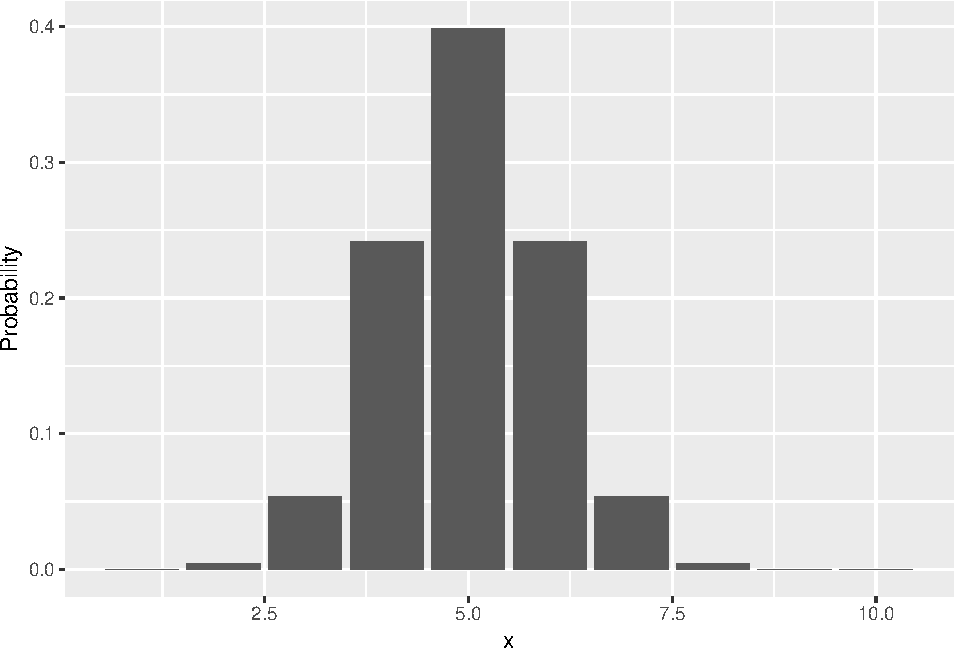
\includegraphics{Biostatistics_files/figure-latex/unnamed-chunk-29-1.pdf}

\section{Central limit theorem}\label{central-limit-theorem}

The central limit theorem establishes that the distribution of sample
means of an independent random variable tends toward a normal
distribution even if the original variables themselves are not normally
distributed. For example, suppose that a sample is obtained containing a
large number of observations, each observation being randomly generated
in a way that does not depend on the values of the other observations,
and that the arithmetic mean of the observed values is computed. If this
procedure is performed many times, the central limit theorem says that
the computed values of the mean will be distributed according to a
normal distribution.

\section{Test for normality}\label{test-for-normality}

The Shapiro-Wilk test of normality tests if the population is normally
distributed. If the p-value is less than a chosen alpha, then the null
hypothesis is rejected and there is evidence that the data tested are
\emph{not} from a normally distributed population. If the p-value is
greater than a chosen alpha, then the data \emph{may} be normally
distributed and one cannot reject the hypothesis that the sample comes
from a population which has a normal distribution.

\begin{Shaded}
\begin{Highlighting}[]
\CommentTok{# Import dataset}
\KeywordTok{load}\NormalTok{(}\StringTok{"docs/Example-data.Rda"}\NormalTok{)}

\CommentTok{# Shapiro-Wilk test of normality}
\KeywordTok{shapiro.test}\NormalTok{(data}\OperatorTok{$}\NormalTok{Age)}
\end{Highlighting}
\end{Shaded}

\begin{verbatim}

    Shapiro-Wilk normality test

data:  data$Age
W = 0.93058, p-value = 0.1584
\end{verbatim}

\section{Quantile-quantile plot}\label{quantile-quantile-plot}

Quantile-quantile (Q-Q) plot is a probability plot, which is a graphical
method for comparing two probability distributions by plotting their
quantiles against each other. If the two distributions being compared
are similar, the points in the Q--Q plot will approximately lie on the
line y = x. If the distributions are linearly related, the points in the
Q--Q plot will approximately lie on a line, but not necessarily on the
line y = x.

\begin{Shaded}
\begin{Highlighting}[]
\CommentTok{# Q-Q plot}
\KeywordTok{library}\NormalTok{(ggplot2)}
\KeywordTok{ggplot}\NormalTok{(data, }\KeywordTok{aes}\NormalTok{(}\DataTypeTok{sample =}\NormalTok{ Age)) }\OperatorTok{+}\StringTok{ }
\StringTok{  }\KeywordTok{stat_qq}\NormalTok{() }\OperatorTok{+}\StringTok{ }
\StringTok{  }\KeywordTok{stat_qq_line}\NormalTok{()}
\end{Highlighting}
\end{Shaded}

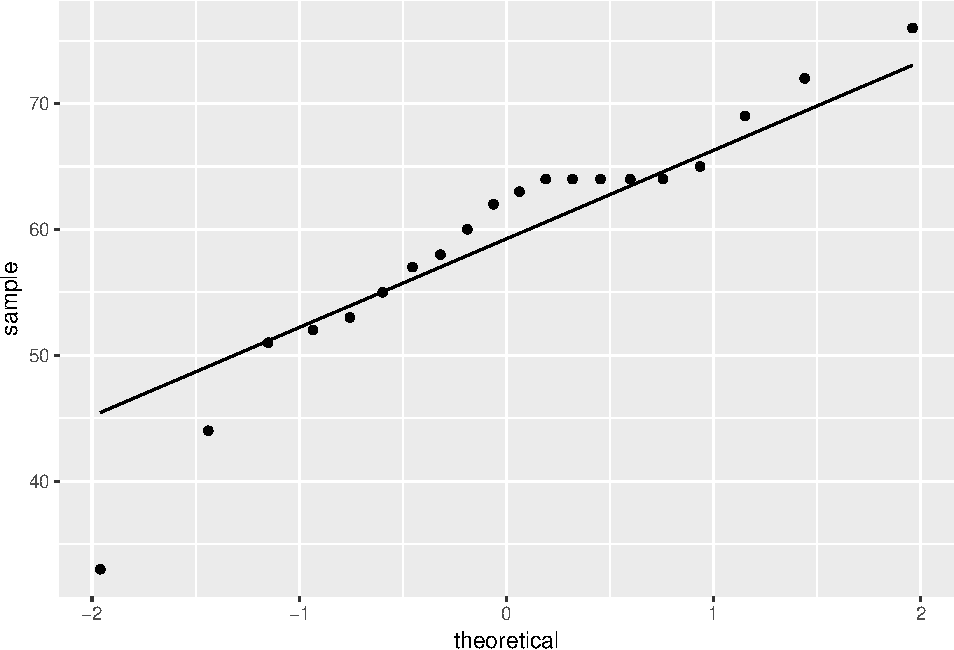
\includegraphics{Biostatistics_files/figure-latex/unnamed-chunk-31-1.pdf}

\section{Confidence interval}\label{confidence-interval}

The interval of plausible estimates of the sample mean is known as the
confidence interval. Generally, the interval encompasses 95\% of all
such sample means. It is calculated from Student's \({t}\) distribution
which is a family of distributions indexed by a parameter referred to as
the degrees of freedom (\({n-1}\)). The upper and lower bounds of the
interval are calculated as follows when the standard deviation of the
population is unknown:
\[{(\bar{x}-t_{n-1,1-\alpha/2}s/\sqrt{n}, \bar{x}+t_{n-1,1-\alpha/2}s/\sqrt{n})}\]
where \(t_{n-1,1-\alpha/2}\) is the the percentage points of the \({t}\)
distribution for a given degree of freedom (\({n-1}\)) and percentile
(\(1-\alpha/2\)). The length of the confidence interval is therefore
proportional to the sample size (\({n}\)), standard deviation (\({s}\)),
and confidence (\(\alpha\)):

\begin{itemize}
\tightlist
\item
  As the sample size increases, the length of the confidence interval
  decreases
\item
  As the standard deviation increases, the length of the confidence
  interval increases
\item
  As the confidence desired increases, the length of the confidence
  interval increases
\end{itemize}

\begin{Shaded}
\begin{Highlighting}[]
\CommentTok{# Determine the confidence interval of the mean from a t distriubtion}
\NormalTok{alpha =}\StringTok{ }\FloatTok{0.05}
\NormalTok{mean =}\StringTok{ }\KeywordTok{mean}\NormalTok{(data}\OperatorTok{$}\NormalTok{Age)}
\NormalTok{sd =}\StringTok{ }\KeywordTok{sd}\NormalTok{(data}\OperatorTok{$}\NormalTok{Age)}
\NormalTok{n =}\StringTok{ }\KeywordTok{length}\NormalTok{(data}\OperatorTok{$}\NormalTok{Age)}
\NormalTok{CI =}\StringTok{ }\KeywordTok{qt}\NormalTok{(}\DataTypeTok{p =} \DecValTok{1}\OperatorTok{-}\NormalTok{alpha}\OperatorTok{/}\DecValTok{2}\NormalTok{, }\DataTypeTok{df =}\NormalTok{ n}\OperatorTok{-}\DecValTok{1}\NormalTok{)}\OperatorTok{*}\NormalTok{sd}\OperatorTok{/}\KeywordTok{sqrt}\NormalTok{(n)}
\KeywordTok{c}\NormalTok{(mean }\OperatorTok{-}\StringTok{ }\NormalTok{CI, mean }\OperatorTok{+}\StringTok{ }\NormalTok{CI)}
\end{Highlighting}
\end{Shaded}

\begin{verbatim}
[1] 54.93078 64.06922
\end{verbatim}

\bibliography{Citations.bib}


\end{document}
